%
% rewriting open objects
% a motivating example
%

% --- comment out when compiling ---
%%
%	rewriting open objects
%	style
%	

%
%  packages
%

\usepackage{amsfonts}
\usepackage{amssymb}  
\usepackage{amsthm} 
\usepackage{amsmath} 
\usepackage{caption}
\usepackage[inline]{enumitem}
	\setlist{itemsep=0em, topsep=0em, parsep=0em}
	\setlist[enumerate]{label=(\alph*)}
\usepackage{doi}
\usepackage{etoolbox}
\usepackage[]{hyperref}
%	\definecolor{hyperrefcolor}{rgb}{0,0,0.7}
	\hypersetup{colorlinks,linkcolor={blue},citecolor={blue},urlcolor={blue}}
\usepackage{graphicx}
	\graphicspath{ {images/} }
\usepackage{mathtools}
\usepackage[numbers]{natbib}
\usepackage{stmaryrd} 
\usepackage{subcaption}
\usepackage{subfiles}
\usepackage{tikz}
	\usetikzlibrary{matrix,arrows,shapes,decorations.markings,decorations.pathreplacing}
\usepackage{todonotes}
\usepackage{url}
\usepackage{xcolor}

%
% commands
%

\newcommand{\RR}{\mathbb{R}}
\newcommand{\ZZ}{\mathbb{Z}}
\newcommand{\NN}{\mathbb{N}}
\newcommand{\QQ}{\mathbb{Q}}
\newcommand{\CC}{\mathbb{C}}
\newcommand{\DD}{\mathbb{D}}
\newcommand{\MM}{\mathbb{M}}
\renewcommand{\epsilon}{\varepsilon}

\newcommand{\Set}{\cat{Set}}
\newcommand{\Graph}{\cat{Graph}}
\newcommand{\RGraph}{\cat{RGraph}}
\newcommand{\Top}{\cat{Top}}
\newcommand{\Cat}{\cat{Cat}}
\newcommand{\A}{\cat{A}}
\newcommand{\B}{\cat{B}}
\newcommand{\C}{\cat{C}}
\newcommand{\X}{\cat{X}}
\newcommand{\Y}{\cat{Y}}
\newcommand{\Z}{\cat{Z}}
\newcommand{\core}[1]{\mathbf{core}(#1)}

\newcommand{\defn}[1]{\textbf{#1}}
\newcommand{\op}[1]{\operatorname{#1}}
\newcommand{\cat}[1]{\mathbf{#1}}
\newcommand{\dblcat}[1]{\mathbb{#1}}
\renewcommand{\t}[1]{\text{#1}}


\newcommand{\from}{\colon}
\newcommand{\xto}[1]{\xrightarrow{#1}}
\newcommand{\sm}{\smallsetminus}
\newcommand{\tospan}{\xrightarrow{\mathit{sp}}}
\newcommand{\tocospan}{\xrightarrow{\mathit{csp}}}
\newcommand{\diagram}[1]{\raisebox{-0.5\height}{\includegraphics{#1}}}

\newcommand{\Sp}[1]{\mathbf{Sp}(#1)}
\newcommand{\MonSp}[1]{\mathbf{MonSp}(#1)}
\newcommand{\SSp}[1]{\mathbb{S}\mathbf{p}(#1)}
\newcommand{\Csp}[1]{\mathbf{Csp}(#1)}
\newcommand{\CCsp}[1]{\mathbb{C}\mathbf{sp}(#1)}
\newcommand{\SpSp}[1]{\mathbf{Sp}(\mathbf{Sp}(#1))}
\newcommand{\SSpSp}[1]{\mathbb{S}\mathbf{p(\mathbf{Sp}(#1))}}
\newcommand{\CspCsp}[1]{\mathbf{Csp}(\mathbf{Csp}(#1))}
\newcommand{\CCspCsp}[1]{\mathbb{C}\mathbf{sp}(\mathbf{Csp}(#1))}
\newcommand{\MonSpCsp}[1]{\mathbf{MonicSp}(\mathbf{Csp}(#1))}
\newcommand{\MMonSpCsp}[1]{\mathbb{M}\mathbf{onicSp}(\mathbf{Csp}(#1))}
\newcommand{\EpCspSp}[1]{\mathbf{EpicCsp}(\mathbf{Csp}(#1))}
\newcommand{\EEpCspSp}[1]{\mathbb{E}\mathbf{picCsp}(\mathbf{Sp}(#1))}
\newcommand{\SpCsp}[1]{\mathbf{Sp}(\mathbf{Csp}(#1))}
\newcommand{\SSpCsp}[1]{\mathbb{S}\mathbf{p}(\mathbf{Csp}(#1))}

\newcommand{\FuncCsp}[1]{ #1 \t{-} \mathbf{Csp}}
\newcommand{\OpenOb}[1]{ #1 \t{-} \mathbf{Open} }
\newcommand{\Rewrite}[1]{ #1 \t{-} \mathbf{Rewrite} }
\newcommand{\RRewrite}[1]{ #1 \t{-} \mathbb{R}\mathbf{ewrite} }
\newcommand{\MonRewrite}[1]{ #1 \t{-} \mathbf{MonRewrite} }
\newcommand{\MMonRewrite}[1]{ #1 \t{-} \mathbb{M}\mathbf{on}\mathbb{R}\mathbf{ewrite} }

%
% math operators
%

\DeclareMathOperator{\Hom}{Hom}
\DeclareMathOperator{\id}{id}
\DeclareMathOperator{\ob}{Ob}
\DeclareMathOperator{\arr}{arr}
\DeclareMathOperator{\im}{im}
\DeclareMathOperator{\Aut}{Aut}
\DeclareMathOperator{\Bij}{Bij}
\DeclareMathOperator{\Sub}{Sub}
\DeclareMathOperator{\colim}{colim}

%
% envirnments and counters
%

\newtheorem{thm}{Theorem}[section]
\newtheorem{lem}[thm]{Lemma}
\newtheorem{prop}[thm]{Proposition}
\newtheorem{cor}[thm]{Corollary}

\theoremstyle{remark}
	\newtheorem{remark}[thm]{Remark}
	\newtheorem{notation}[thm]{Notation}

\theoremstyle{definition}
	\newtheorem{ex}[thm]{Example} 
	\newtheorem{df}[thm]{Definition}

% \setcounter{tocdepth}{1} % Sets depth for table of contents. 

%
% tikz types
%
\tikzset{->-/.style={decoration={%
			markings,
			mark=at position .5 with {\arrow{>}}},postaction={decorate}}
}
\tikzset{->-pos/.style={decoration={%
			markings,
			mark=at position #1 with {\arrow{>}}},postaction={decorate}}
}
\tikzset{->-/.style={decoration={%
			markings,
			mark=at position .5 with {\arrow{>}}},postaction={decorate}}
}
\tikzset{->-pos/.style={decoration={%
			markings,
			mark=at position #1 with {\arrow{>}}},postaction={decorate}}
}

%
% inline diagrams
%
\newcommand{\rgraph}[2]{%
	$\begin{tikzpicture}
	\node (a) at (0,0) {$ #1 $};
	\node (b) at (1,0) {$ #2 $};
	\draw [->] (a.30) to (b.150);
	\draw [->] (a.-30) to (b.-150);
	\draw [->] (b) to (a);
	\end{tikzpicture}$
}
\newcommand{\graph}[2]{%
	$\begin{tikzpicture}
	\node (a) at (0,0) {$ #1 $};
	\node (b) at (1,0) {$ #2 $};
	\draw [->] (a.30) to (b.150);
	\draw [->] (a.-30) to (b.-150);
	\end{tikzpicture}$
} % input preamble
%\bibliography{} % input bibliograph	

\documentclass[master_reopn]{subfiles}
\begin{document}

\section{A motivating example} \label{sec_motivating-example}

This section serves two functions. First, we discuss the example that motivates this paper.  Within our discussion, we take the opportunity to set both notation and language used in the sequel.  

When reading network theory literature written from the compositional perspective, one comes across the notion of an open graph. 
	\todo{cite}
The level of formality this definition is given varies between authors, but the core idea is that an \emph{open graph} is a $ \Set $-diagram $ E \rightrightarrows N $ together with a subset $ L \subseteq N$ equipped with a partition $ L = L_{ \t{in} } + L_{ \t{out} } $.
	\todo{insert diagram D1-open graph}
The conceit is that the subset of nodes $ L $ is a boundary that is accessible to other open graphs. Elements of $ L_{ \t{in} } $ and $ L_{ \t{out} } $ are thought of as inputs and outputs, respectively.  Given two open graphs $ (E \rightrightarrows N , L_{ \t{in} } + L_{ \t{out} }) $ and $ (E' \rightrightarrows N' , L'_{ \t{in} } + L'_{ \t{out} }) $, such that $ L_{ \t{out} } = L'_{ \t{in} } $, then we can construct the graph $ (E + E' \rightrightarrows (N + N') / L_{ \t{out} } = L'_{ \t{in} } ,  L_{ \t{in} } + L'_{ \t{out} } ) $.  For example,
	\todo{insert diagram D2-glueing open graphs}.
We casually add that by appropriately modifying the definition of a graph morphism, one can define a morphism of open graphs.

A primary motivation behind this construction is to model the process of connecting networks together.  Although, some networks contain additional information that cannot be conveyed by an open graph as described above.
	\todo{cite examples: circ, zx-calc, petri nets, etc}
To accommodate such demands, we generalize the notion of an open graph to that of an \emph{open object} and develop some basic theory for open objects.  

One feature that distinguishes this work from other related work is our preference for reflexive graphs over directed graphs.  Before mentioning our reasons, let us clarify exactly what we mean by these two sorts of graphs. Denote by $ \rgraph{\bullet}{\bullet} $ the category with two objects $ [0] $ and $ [1] $ with two arrows $ s,t \from [1] \to [0] $ and an arrow $ r \from [0] \to [1] $ that is a section to both $ s $ and $ t $.  Throughout this text, the category of reflexive graphs is $ \RGraph \coloneqq [ \rgraph{\bullet}{\bullet} , \Set] $ and the category of directed graphs is $ \Graph \coloneqq [ \graph{\bullet}{\bullet} , \Set ] $.  The reasons for working with reflexive graphs are myriad.  For one, elements $ 1 \to \Gamma $ of a graph $ \Gamma $ are not just nodes, but nodes with a loop attached.  It follows that the underlying nodes functor $ \RGraph \to \Set $ is representable by the terminal graph. This is not the case for the underlying nodes functor of type $ \Graph \to \Set $.  Also, the objects of $ \RGraph $ are truncated simplicial sets. The advantage of this goes, perhaps, beyond the scope of this paper. Suffice to say, when working with graph relations, particularly those homotopical in nature, we desire a well-known model structure to work with.  Having said this, let it be known that from this point, any reference to a ``graph'' will mean a ``reflexive graph'' unless specified otherwise. This includes cases when we modify ``graph'' with an adjective. For instance, by ``open graph'' we actually mean ``open reflexive graph''.

Because open graphs are the archetypal example of an open object, it behooves us to formalize that which we have so far glossed over. 

\begin{df} \label{df:OpenGraph}
	Let $ L \from \Set \to \RGraph $ be the discrete graph functor.  An \textbf{open graph} is a cospan of the form $ L x \to \gamma \gets L y $.  
\end{df}

In this definition, there is a graph $ \gamma $ with input nodes $ Lx $ and output nodes $ Ly $.  The functor $ L $ allows us to simultaneously treat graph boundaries $ Lx + Ly $ as both separate from and part of the graph.  

Immediately emerging are two perspectives on open graphs, both alluded to above. The first we call \emph{the structured cospan perspective}. From this point of view, we want to be able to glue together suitable open graphs to form new open graphs. This leads one to consider a category with sets as objects as with open graphs $ Lx \to \gamma \gets Ly $ as arrows of type $ x \to y $.  Composition uses pushouts as is typical in cospan categories.
Heuristically, pushing out can be thought of as a ``categorical gluing''. 
\todo{ref diagram abv?}
 The second perspective is called the \emph{open object perspective}.  Here, we treat open graphs as mathematical objects deserving of their own morphisms.  Indeed, a morphism 
\[
(L x \to \gamma \gets L y) \to ( L x' \to \gamma' \gets L y' )
\]
of open graphs is a a commuting diagram
\[
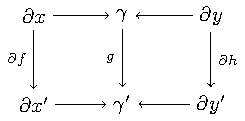
\includegraphics{diag_open-graph-morph_reopn}
\]
This leads to another category where open graphs are objects, as opposed to arrows.  

Having two categories featuring open graphs---one as arrows, the other as objects---one can construct a double category containing all of this structure.  This double category is defined to have sets as 0-cells, set functions as vertical 1-cells, open graphs as horizontal 1-cells and morphisms of open graphs as 2-cells.  The composition functor of this double category takes advantage of the fact that open graphs are also arrows of a category.  
\todo{include D4 composition diagram}
Later, we prove that this actually forms a double category. 




In fact, we do this in Section BLAH. 
	\todo{input appropriate section}
In the following section, we generalize open graphs to `open objects' and construct a pair of categories, one with open objects as arrows and the other with open objects as objects.  

\end{document}



